\documentclass[10pt,a4paper]{article}
\usepackage[margin=19mm]{geometry}
\usepackage{amsmath,amssymb,graphicx,booktabs,hyperref}
\hypersetup{colorlinks=true,urlcolor=blue}
\setlength{\parindent}{0pt}
\setlength{\parskip}{5pt}
\begin{document}
\begin{center}
{\Large\bfseries Guarded coefficient circuits for original Curve25519 sections}\\[4pt]
2026-11-23 \quad Source PR5040 \quad Producer evidence, unsigned/unverified
\end{center}

The compiler keeps five normalized section coefficients unknown and emits
acyclic quadratic equations over $\mathbb F_p$, with two forced inverse inputs.
Its arguments are public Spec,$R,Q=[8]R$ only. Known coefficients enter a
separate extension control, followed by projection and the unchanged original
indexed extractor and group replay. Statements: PCC-20261123-70247b (written)
and PCC-20261123-7f4e38 (native), both unsigned. [pcc:unverified]

\textbf{Construction and precise domain.}
Use the original norm-section chart: $c_4=1$ for finite $R$ with nonzero
ordinate, or $c_5=1$ for $R=O$. This leaves five coefficients and a monic
sextic $S$. Put $r_0=-A/2$ and $S=(X-r_0)B+S(r_0)$. The guarded map is
\[
 \beta S(r_0)=1,\qquad \lambda=-(A/2)\beta B\pmod S.
\]
No unknown inverse is evaluated freely. For declared rational nonzero-ordinate
support, the classical Montgomery doubling formula yields
\[
 J_A=(X-1)\big((X^2-1)^2-4(X^3+AX^2+X)\big),\qquad
 \eta\det(M_{J_A})=1.
\]
Here $M_{J_A}$ is multiplication by $J_A$ in $\mathbb F_p[X]/S$.
The hypotheses $A+2$ square and $A-2$ nonsquare give unique rational nonzero
2-torsion and only the $x=1$ rational order-4 branch. On this support,
$J_A(x(P))=0$ iff $[8]P=O$. The degree-five guard replaces the old degree-63
denominator under these hypotheses; the membership condition remains.
This is a written argument with fixed native checks, not a formal torsion or
compiler theorem. [pcc:unverified]

\begin{center}
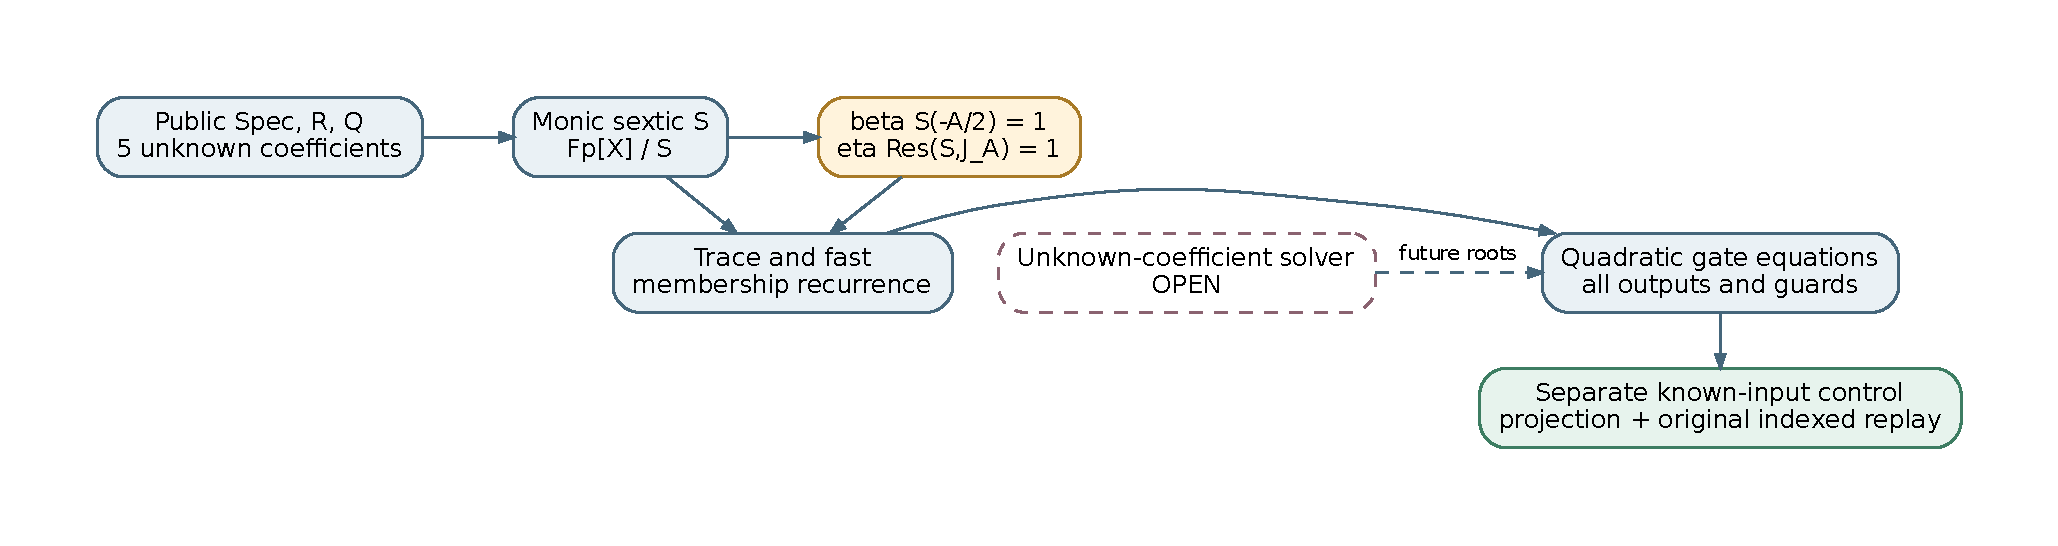
\includegraphics[width=\linewidth]{pipeline.pdf}
\end{center}
\textbf{Figure 1.} Guarded circuit and separate known-input control. Unknown
root discovery is an open component, shown dashed.

Compile $\tau=4T_q(\lambda)^2-2$ and the frozen fast finite-free geometric
product recurrence. Every final field coordinate, norm forced-factor remainder
and inverse guard remains constrained. Each gate has its own equation such as
$z-a-b=0$ or $z-ab=0$. Topological induction gives the written extension/
projection construction over $\mathbb F_p$. Seven input wires do not mean
seven total variables; quadratic gate degree does not bound solving degree.
Algebraic-closure filtering and original lifting remain obligations.

\textbf{Exact original parameters.}
$p=2^{255}-19$, $A=486662$, $a=60824497$, $q=213156431$.
The toy is $p=101,A=95,a=17,q=3,k=8$. Fixed primality/exact-order context is
inherited; no new curve certificate or twist transfer is asserted.

\newpage
\textbf{Fixed controls and representation counts.}
One qualified local native call used a 600-second wall cap and 2,GiB virtual
memory cap: 15 planned, 15 attempted, 15 completed, zero excluded; 16 JSONL
records include completion. Four focused release tests, fmt and strict
all-target Clippy passed after retained failed build/lint attempts.
[pcc:unverified]

\begin{center}
\begin{tabular}{lrr}
\toprule
Original actual-$q$ fixture & Variables & Equations\\
\midrule
$k=31$ & 41,493 & 41,514\\
$k=20,633$ & 4,597,568 & 4,597,589\\
\bottomrule
\end{tabular}\\[4pt]
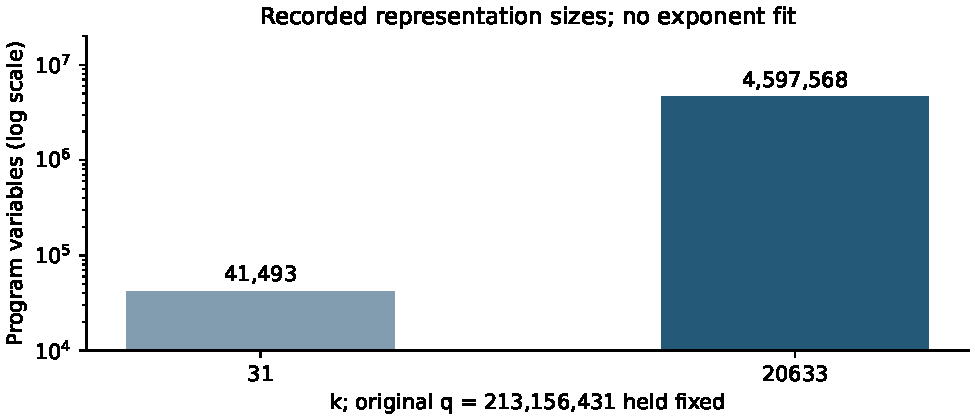
\includegraphics[width=.86\linewidth]{counts.pdf}
\end{center}
\textbf{Figure 2.} One deterministic program per fixed $k$, with actual $q$
and known section held fixed. No sampling interval applies. Counts are not
timing, normalized field work, peak RAM or a fitted growing-family exponent.

Controls include eight toy sign patterns, two identity-$R$ sections, all 101
$c_3$ pencil values (one accepted and originally replayed), all 102 rational
nonzero-ordinate toy points and six actual signed low-order points for the
torsion check, 64 distributed wire increments plus two inverse-input mutations,
and malformed/resource refusals. Both actual cases use the original $q$ and
known $j=1,\ldots,6,t=0$ section. Coefficients were supplied to extension;
this is not public-target coefficient discovery. [pcc:unverified]

\textbf{Provenance and publication.}
Local source \texttt{6f4987bd} preceded the call; public source
\texttt{e1591a20} has identical source blobs. The 54-input context comprises
unchanged 30- and 11-input archives plus the 13-input, 21,360-byte delta.
Ten compiled-in hashes, all source hashes and immutable binary
\texttt{46e75f76} match before/after. The full archive is 117,571,164 bytes,
SHA256 prefix \texttt{697a904ccfda}; raw 218,010 bytes/
\texttt{e9d3ccf6a00b} and all 24 full program/assignment exports remain local.
Trusted-store publication is pending. Metadata hashes are not signed execution
or remote-availability receipts. [pcc:unverified]

\textbf{Decisive next step.}
Discover unknown coefficients on the same guarded predicate, then charge full
setup, solving, field filtering, useful yield, selection/rank, indexing,
recovery and memory on a declared growing family. The current compiler makes
that input problem explicit. No canonical performance/leaderboard datum is
admitted by this construction. The proof map names formal gaps, including the
absence of a new identity certificate or native compiler proof.

{\small\sloppy\textbf{Evidence and primary sources.}
Study: \path{section-compiler-v1/PROTOCOL.md}, \path{DERIVATION.md},
\path{PROOF_MAP.md}, \path{SOURCE_QUALIFICATION.json},
\path{native-v1/SUMMARY.json}, \path{ARCHIVE.json}.\\
Costello--Smith, \emph{Montgomery curves and their arithmetic}, sections 2.3/3.3,
\url{https://arxiv.org/html/1703.01863v1}.\\
EFD Montgomery XZ formulas:\\
\url{https://hyperelliptic.org/EFD/g1p/auto-montgom-xz.html}.\\
Macaulay2 determinant-strategy documentation; frozen original quotient-query
recurrence and section-coeff-v1 derivation. KB/ecdb access gaps and failed
fetches are recorded; no novelty clearance is asserted.}
\end{document}
